%! TEX program = luatex
\documentclass[11pt]{article}
\usepackage{textcomp}
\usepackage{graphicx,wasysym, mdframed,xcolor,gensymb,verbatim}
\usepackage{color}
\usepackage{floatflt}

\usepackage[italian]{babel}
%%se si usa pdflatex:
%\usepackage[utf8]{inputenc}
%\usepackage[scaled=0.9]{FiraSans}
%
%i seguenti comandi funzionano con lualatex (si possono usare tutti i font di sistema come in vim o nel terminale!)
\usepackage{fontspec}
%\setmonofont{Inconsolatazi4}
%
% 0 OfficeCodePro 1=inconsolata 2=Hack
\ifcase 0 %font 0
\setmonofont[Scale=0.7,
  ItalicFont=OfficeCodePro-RegularItalic,
  BoldFont=OfficeCodePro-Bold,
  BoldItalicFont=OfficeCodePro-BoldItalic,
  UprightFont=OfficeCodePro-Regular]
  {OfficeCodePro}
\or% font 1
\setmonofont[Scale=0.7,
  ItalicFont=inconsolatalgcitalic,
  BoldFont=inconsolatalgcbold,
  BoldItalicFont=inconsolatalgcitalic,
  UprightFont=inconsolatalgc]
  {inconsolatagc}
\else% else
%
%imposto il font per listings (si possono anche indicare le varianti, i.e. italic, bold, bolditalic)
\setmonofont[Scale=0.7,
  ItalicFont=Hack-Italic,
  BoldFont=Hack-Bold,
  BoldItalicFont=Hack-BoldItalic,
  UprightFont=Hack-Regular]
  {Hack}
\fi
%
\usepackage[T1]{fontenc}
% un'alternativa a listingsutf8 è il pacchetto minted ma richiede una libreria python chiamata Pygments
\usepackage{listingsutf8}
\definecolor{verdeoliva}{rgb}{0.3,0.3,0}
\definecolor{grigio}{rgb}{0.5,0.5,0.5}
\definecolor{blumarino}{rgb}{0.0,0,0.5}
\definecolor{panna}{rgb}{0.98,0.98,0.94}
\def\lstlistingname{Listato}
\lstset{%
  %inputencoding=utf8,
  breaklines=true,
  %extendedchars=true,              % lets you use non-ASCII characters; for 8-bits encodings only, does not work with UTF-8
  %literate=%
  %       {á}{{\'a}}1
  %       {í}{{\'i}}1
  %       {é}{{\'e}}1
  %       {ý}{{\'y}}1
  %       {ú}{{\'u}}1
  %       {ó}{{\'o}}1,
  backgroundcolor=\color{panna},   % choose the background color; you must add \usepackage{color} or \usepackage{xcolor}; should come as last argument
% basicstyle=\footnotesize\ttfamily,
  basicstyle=\ttfamily,            % è selezionato all'inizio di ogni listing
  belowskip=-0.2\baselineskip,
% basicstyle=\footnotesize,        % the size of the fonts that are used for the code
  breakatwhitespace=false,         % sets if automatic breaks should only happen at whitespace
% breaklines=true,                 % sets automatic line breaking
  captionpos=b,                    % sets the caption-position to bottom
  commentstyle=\itshape\color{verdeoliva}, % comment style (nota: all'inizio del listing seleziona \ttfamily, perciò qui seleziona la variante italic)
% deletekeywords={},            % if you want to delete keywords from the given language
% escapeinside={\%*}{*)},          % if you want to add LaTeX within your code
% firstnumber=1000,                % start line enumeration with line 1000
  frame=single,	                   % adds a frame around the code
  keepspaces=true,                 % keeps spaces in text, useful for keeping indentation of code (possibly needs columns=flexible)
  keywordstyle=\bfseries\color{blue},       % keyword style
% language=Octave,                 % the language of the code
% morekeywords={*,},            % if you want to add more keywords to the set
  numbers=left,                    % where to put the line-numbers; possible values are (none, left, right)
  numbersep=5pt,                   % how far the line-numbers are from the code
  numberstyle=\tiny\color{grigio}, % the style that is used for the line-numbers
  rulecolor=\color{black},         % if not set, the frame-color may be changed on line-breaks within not-black text (e.g. comments (green here))
  showspaces=false,                % show spaces everywhere adding particular underscores; it overrides 'showstringspaces'
  showstringspaces=false,          % underline spaces within strings only
  showtabs=false,                  % show tabs within strings adding particular underscores
  stepnumber=1,                    % the step between two line-numbers. If it's 1, each line will be numbered
  stringstyle=\color{blumarino},   % string literal style
  tabsize=2,	                   % sets default tabsize to 2 spaces
  title=\lstname%                  % show the filename of files included with \lstinputlisting; also try caption instead of title
}



%%%%%%%%%%%%%%%%%%%%%
\usepackage{listings}
\usepackage{xcolor}
\usepackage{bm}

%New colors defined below
\definecolor{codegreen}{rgb}{0,0.6,0}
\definecolor{codegray}{rgb}{0.5,0.5,0.5}
\definecolor{codepurple}{rgb}{0.58,0,0.82}
\definecolor{backcolour}{rgb}{0.95,0.95,0.92}

%Code listing style named "mystyle"
\lstdefinestyle{mystyle}{
  backgroundcolor=\color{backcolour},   commentstyle=\color{codegreen},
  keywordstyle=\color{magenta},
  numberstyle=\tiny\color{codegray},
  stringstyle=\color{codepurple},
  basicstyle=\ttfamily\footnotesize,
  breakatwhitespace=false,         
  breaklines=true,                 
  captionpos=b,                    
  keepspaces=true,                 
  numbers=left,                    
  numbersep=5pt,                  
  showspaces=false,                
  showstringspaces=false,
  showtabs=false,                  
  tabsize=2
}
\lstset{style=mystyle}
%%%%%%%%%%%%%%%%%%%

\newcommand{\voto}[1]{[\textbf{#1} punti]}
\def\cmu{\mbox{cm$^{-1}$}}
\def\half{\frac{1}{2}}

\voffset -2cm
\hoffset -2.5cm
%\marginparwidth 0cm
\textheight 22cm
\textwidth 17cm
%\oddsidemargin  0.2cm                                                                                         
%\evensidemargin 0.4cm                                                                                         
\parindent=0pt

\begin{document}
\pagestyle{empty}

\begin{center}
{\Large \bf  Laboratorio di Calcolo per Fisici, Terza esercitazione\\[2mm]}
{\large Canale D-K, Docente: Livia Soffi, Esercitatori: Prof. S. Rahatlou e Prof. R. Faccini}
\end{center}
\vspace{4mm}

\colorbox{yellow}{\begin{minipage}{17cm}
  Lo scopo della terza esercitazione di laboratorio \`e di scrivere da zero un programma che utilizzi, a seconda delle necessit\`a i tre costrutti principali: \textbf{operazioni-scelte decisionali-iterazioni}.
\end{minipage}}
\vspace{2mm}
%\vspace{1mm}
%
%

\hrule
\vspace{2mm}
\vspace{2mm}
\textbf{$\RHD$ Prima parte (obbligatoria)} 
Lo scopo di questa prima parte \`e quello di realizzare da zero un programma che  sia in grado di studiare figure geometriche standard, i \textbf{poligoni regolari}. Tali poligoni hanno la caratteristica di avere $n$ lati e $n$ angoli uguali tra loro. Possono essere inscritti e circoscritti in circonferenze i cui raggi possono essere ricavati tramite semplici relazioni matematiche a partire da $n$ e dal valore del lato $l$ del poligono [vedi formulario ultima pagina]. Ci concentriamo qui sui poligoni regolari con \textbf{$\bm{n}$ compreso tra 3 e 10}. 

\begin{enumerate}
\item Fare login sul computer e aprire una finestra di {\em terminale}.
\item Creare nella vostra \emph{home} una cartella  \textbf{EX3} in cui lavorare per l'intera esercitazione.
\item Nella cartella EX3 aprire con l'editor  di testo \emph{emacs} il file \textbf{poligoni.c} in cui dovrete implementare il programma.
\item Come prima cosa il programma deve chiedere all'utente di inserire il giorno, il numero,  il mese e l'anno della data odierna e dovr\`a poi stamparlo nel seguente formato "Oggi è [giorno] [XX] [mese] [YYYY]". Per farlo utilizzare le funzioni \emph{\textbf{scanf}} e \emph{\textbf{printf}} e gli opportuni descrittori.

\item Il programma dovr\`a poi chiedere all'utente di inserire il numero $n$ di lati del poligono regolare che si vuole studiare e il valore $l$ del lato. Inserire un controllo in modo tale che se il numero inserito non \`e compreso tra 3 e 10 l'utente sia invitato a inserire di nuovo il numero. Per farlo utilizzare il costrutto \emph{\textbf{do.. while}}

\item Calcolare e stampare, accompagnati da opportune stringhe di testo esplicative:

- il valore del numero fisso $N$ 

- il valore dell'apotema, o raggio della circonferenza inscritta, $r$

- il valore del perimetro $P$ 

- il valore dell'area $S$ del poligono

- il valore del raggio $R$ della circonferenza circoscritta al poligono 

\item Ripetere il punto precedente modificando il programma in modo tale che venga chiesto all'utente quale delle cinque grandezze calcolare. Per farlo utilizzare il costrutto \emph{\textbf{if.. else}}

\item Modificare ulteriormente il programma in modo che questo, una volta chiesto il valore del lato, calcoli automaticamente: il numero fisso, l'apotema, il perimetro e l'area per per ciascun valore $n$ di lati da 3 a 10. Per farlo utilizzare il costrutto \emph{\textbf{for(..)}}

\item Scrivere su un file \emph{output.dat} i valori di $n$, $N$, $a$, $P$, $S$ e $R$ su cinque colonne.
\end{enumerate}

NB. Si ricorda che per compilare ed eseguire il programma in C si deve digitare sul terminale:

\colorbox{yellow}{\begin{minipage}{17cm}
  gcc poligoni.c -o poligoni.x \\
  ./poligoni.x
\end{minipage}}

\hrule
\vspace{2mm}
\textbf{$\RHD$ Seconda parte (obbligatoria)} 
 Graficare, tramite uno script in python analogo a quelli utilizzati nelle EX1 e EX2, il numero fisso, l'apotema, il perimetro e l'area in funzione del numero di lati. Salvare le immagini cosi` ottenute. Si riporta per completezza un template dello script da utilizzare. 
%\begin{mdframed}[backgroundcolor=panna]
\begin{lstlisting}[language=Python, caption=Python example]
#!/usr/bin/env python3

import matplotlib.pyplot as plt
import numpy as np

plt.title('Un primo plot con Python')
plt.xlabel('numero di lati')
plt.ylabel('N')
x, y = np.loadtxt('output.dat', comments=['#'], usecols=(1,2), unpack=True)
plt.plot(x, y, 'x', label='Numero fisso vs numero di lati')
plt.xlim(0, 12)
plt.ylim(0, 3)
plt.savefig('N_vs_n.png')
plt.show()
# facciamo un reset della figura
plt.clf()
#ora possiamo crearne una nuova 
\end{lstlisting}
\hrule
\vspace{2mm}
\textbf{$\RHD$ Terza parte (facoltativa)} 
Utilizzare le formule del raggio per la circonferenza iscritta e circoscritta ad un poligono per ricavare numericamente \textbf{una stima del $\pi$} scrivendo un programma chiamato \textbf{stima\_pi.c}. 
Si consideri un poligono regolare di $2^n$ lati avente un perimetro di lunghezza fissata uguale a 2. Chiamati con $r_n$ e $R_n$ i raggi rispettivamente del cerchio inscritto nel poligono e del cerchio che lo circoscrive è evidente che il perimetro del poligono risulta maggiore di $2 \pi r_n$ e minore di $2 \pi R_n$. 
Si ha pertanto $2 \pi r_n < 2<  2\pi R_n$
da cui isolando $\pi$ si ottiene :
$$\frac{1}{R_n} <  \pi < \frac{1}{r_n}$$
Scopo del programma deve essere di calcolare $r_n$ e $R_n$ per valori di $n$ crescenti in modo da ottenere una stima inferiore e una superiore al valore di $\pi$ man mano piu' precisa. 

Suggerimento: Utilizzare il seguente algoritmo iterativo [Metodo di Cusano]:
\begin{enumerate}
\item Partire da $n = 2$ si ha $2^n = 4$ ossia  il poligono considerato è un quadrato. Per avere $P=2$ il lato $l$ del quadrato deve essere 0.5.
\item Calcolare $r_2$ e $R_2$ sfruttando il programma \textbf{poligoni.c}. Dovreste ottenere $r_2 = \frac{1}{4}$ e $R_2 = \frac{\sqrt{2}}{4}$
\item Si pu\`o dimostrare che i raggi interni e esterni delle circonferenze relative a poligoni di $2^n$ lati con $n>2$  e perimetro fissato pari a 2 possono esprimersi come:
$$r_{n+1} = \frac{r_n+R_n}{2}$$
$$R_{n+1} =\sqrt{r_{n+1} \cdot  R_{n}}$$
dove $n$ è l’esponente del numero $2^n$
dei lati dei poligoni regolari che approssimano
sempre di più il loro perimetro alle circonferenze dei due cerchi concentrici inscritto e circoscritto al suddetto poligono. 
\item Iterare sul numero dei lati $2^n$ con $n=2,3,4,...$. A ciascun iterazione calcolare $r_n$, $R_n$,$r_{n+1}$, $R_{n+1}$ e la stima superiore e inferiore al $\pi$.  
\item Inserire un opportuno controllo in modo che ad ogni iterazione venga calcolata la differenza tra le stime ottenute e il valore noto del $\pi$. Iterare il calcolo fino a che il valore di $\pi$ ottenuto in entrambi gli estremi \`e compatibile con il valore $3.1415926$ entro un'errore inferiore a $0.0000001$. Quanti lati ha il poligono cos\`i ottenuto?
\item Scrivere, ad ogni iterazione il valore di $n$, estremo superiore, estremo inferiore e relativi errori su un file \textbf{stime.dat}.
\item Graficare utilizzando un'opportuno script in python l'andamento dei due estremi in funzione del numero di lati $n$. 
\item Verificare graficamente che la condizione richiesta al punto precedente sugli errori finali sia effettivamente verificata.
\end{enumerate}



\hrule
\vspace{2mm}
\textbf{$\RHD$ Relazioni Geometriche utili}
\vspace{2mm}


\colorbox{yellow}{\begin{minipage}{10cm}
\begin{itemize}
  \item $N = \frac{1}{2 \cdot tan(\frac{\pi}{n})}$
 \item $r = l \cdot N$
 \item $P = n\cdot l$
  \item $S = \frac{P\cdot r}{2} =  \frac{n\cdot l \cdot r}{2}$

  \item $R=\sqrt{r^2 + \left ( \frac{l}{2} \right ) ^2}$
  \item $l$ = lato del poligono,\\ $n$ = numero di lati,  \\$2p$ = perimetro, \\$S$ = area, \\ $r$ = apotema = raggio del cerchio inscritto,\\$N$ = numero fisso,\\ $R$ = raggio del cerchio circoscritto.
 \end{itemize}
\end{minipage}
    \begin{minipage}{0.5\textwidth}
  %   \begin{figure}[h]
        \begin{center}
        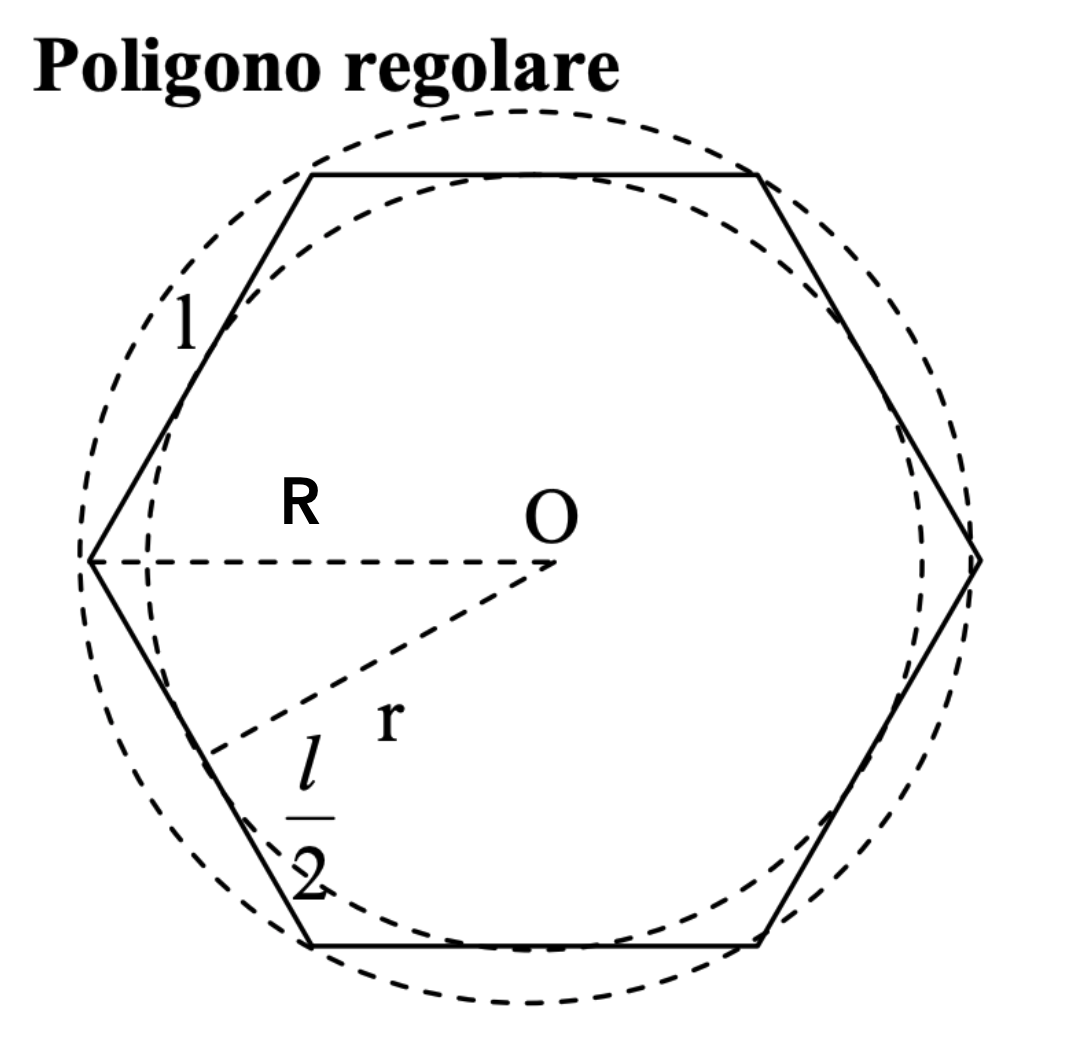
\includegraphics[scale=0.4]{poligono.png}
        \end{center}
   %   \end{figure}
    \end{minipage}}

\end{document}